\section{Theory}
\label{sec:theory}

Early twentieth century observations of atmosphere pressures showed a peculiar
relationship between those measurements in the western tropical Pacific and
those in the southeastern tropical Pacific \citep{holton1989}. Namely, that they
were out of phase --- when one measure was positive, the other was negative.
This was termed the \emph{Southern Oscillation}. Later studies \ref{TODO} would
show that there were accompanying variations in rainfall, sea surface
temperatures, and wind patterns. The combination of these effects would come to
be known collectively as the \elnino{} \emph{Southern Oscillation}, with the
warm phase named \elnino{} and the cold phase \nina{}.


\subsection{Southern Oscillation}
Since the late 19th century, the existence of a large scale `seesaw' in oceanic
surface pressure across the Pacific had been observed \citep{trenberth2000}. The
essence of this observation is that when air pressure is high over the Pacific
Ocean, air pressure tends to be lower over the Indian Ocean (and vice versa)
\citep{philander1990}; from this it was inferred that the two regions were
causally connected by some then-unknown meteorological teleconnection. It was
Walker and Bliss who, in the 1930s, characterised this pattern using measures
% Could/should probably say in more detail how exactly they characterised this
such as sea level pressure and precipitation, naming it the Southern Oscillation
(SO). Walker also defined an index for the SO, calling it the Southern
Oscillation Index (SOI). Figure \ref{fig:slp_corr} shows the average spatial
distribution of SOI correlations for the Pacific, showing the eastern and
western Pacific to be out of phase.
% TODO Some more discussion of indices here. Describe exactly what SOI is,
% describe other indices, particularly ones we use.

\begin{figure*}
  \centering
  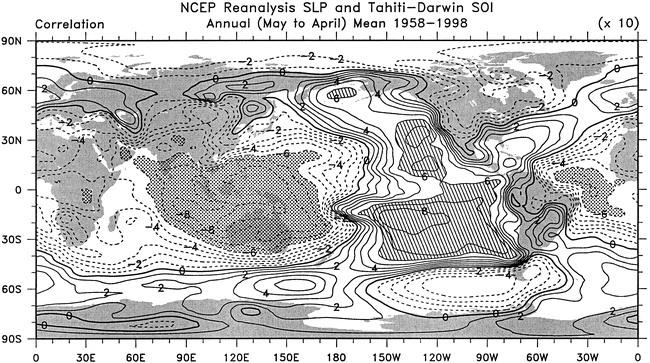
\includegraphics[width=0.75\textwidth]{figures/slp_corr}
  \caption{Sea level pressure correlations with Southern Oscillation Index, a
    measure of the SO devised by Walker. Regions with correlations $>0.6$ are
    hatched and those $<-0.6$ are dotted. It is clear to see that the eastern
    and western tropical Pacific ocean are anticorrelated. Figure taken from
    \cite{trenberth2000}.
    % TODO Is it clear? Maybe this needs more exposition.
  }
  \label{fig:slp_corr}
\end{figure*}

While Walker managed to characterise the atmospheric component of the SO, the
interannual pressure fluctuations driving it were irregular and there was not
enough data for Walker to determine whether the ocean was involved in the
system.

\vspace{0.5cm}

In his seminal 1961 study Bjerknes began formulating a model of how the
interaction of both atmospheric and oceanic components could lead to the
appearance of \elnino{} conditions over the tropical Pacific
\citep{bjerknes1961}. He reasoned that much of the connection lied in weakening
of trade (east-to-west equatorial) winds owing to natural fluctuations caused,
for example, by the uneven solar radiation. The trade winds at the sea surface
drag surface water with them. When the trade winds weaken, the friction between
air and sea surface is reduced, thus allowing warmer western Pacific water to
flow to the cooler east. An abundance of warm water along equatorial South
America then surges into the Peruvian coast, as observed by the Peruvian
fishermen.

Later \citep{bjerknes1966} it was also noted that weakening of the trade winds
would lead to reduced upwelling. The general view of the tropical Pacific is of
relatively warmer waters in the west (near Australia), gradually cooling towards
the east (near Peru). This is typically described as having a thermocline (where
cold water meets warm water) gradually rising from west to east. If the trade
winds weaken the thermocline becomes depressed in the east due to the
aforementioned resurgence of warm water. The anomalous warming of seas then
imparts energy into the atmosphere above. Bjerknes states in his conclusion:
``So much seems certain, however, that the extensive warmings of the East
Pacific equatorial waters are due to a weakening of the equatorial easterly
winds to such an extent that (a) the normal upwelling appreciably weakens of
even ceases'', making the case for an ocean-atmosphere connection.

A key result of \citep{bjerknes1966} is that by using the above reasoning
Bjerknes was able to link strengthening of westerlies in the middle latitudes
occurring with accompanying warming of equatorial ocean water. Bjerknes reasoned
that anomalous warming of surface water would then increase the \emph{Hadley
  circulation} rate, thus leading to increased westerly wind strengths.

The Hadley circulation is the poleward atmospheric circulation of
equatorial air away from the equator. The process is diagrammed in
\ref{fig:hadleycell} and is as follows \citep{geomar6557}. Warm air carried by
the trade winds (moving in an easterly and equatorial direction) converges at
the equator where it releases moisture and rises. The Earth's rotation causes a
Coriolis force which results in the rising air being pushed poleward. The
Coriolis force is clockwise in the Northern hemisphere and anti-clockwise in the
Southern hemisphere; in both cases, as the air moves poleward it also
experiences an eastward motion, whereas at the equator it is moving westward
with the trade winds. Having cooled, the air begins to sink at the upper
latitudes, where the Coriolis force now brings the air back towards the equator,
eventually with an easterly component --- the trade winds.

\begin{figure}[t]
  \centering 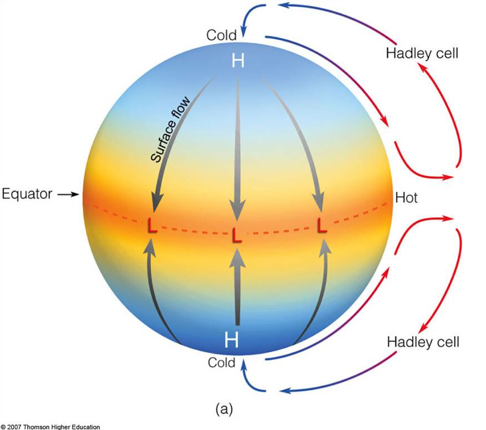
\includegraphics[width=0.9\linewidth]{figures/hadleycell.png}
  \caption{The Hadley circulation. Warm air rises at the equator, is pulled away
    from the equator and towards the poles, cools and falls at greater
    latitudes, then is pulled back towards the equator. This circulation is
    largely created by uneven solar heating and the Coriolis force due to the
    Earth's rotation.}
  \label{fig:hadleycell}
  % From https://www.seas.harvard.edu/climate/eli/research/equable/hadley.html
\end{figure}

Bjerknes continued his investigation into the causes and effects of anomalous
heating in the tropical Pacific ocean and atmospheric pressure variation in his
1969 study \emph{Atmospheric Teleconnections from the Equatorial Pacific}
\citet{bjerknes1969}. In this study a clear connection between \elnino{} and the
SO was demonstrated, particularly that a 1963 \elnino{} event caused a strong
response in the SO.

Figure \ref{fig:pressureprofiles} shows how the dynamic height of a number of
isobars (surfaces of constant atmospheric pressure) varies along the equator
during the months January 1960, and July 1960. In both months it can be seen
that, in the region marking the Pacific ocean, the streamline gradient closest
to the sea surface is towards the west (indicated in \ref{fig:pressureprofiles}
by the line ``S.L.''). Since the streamline gradient shows us how air would move
subject to atmospheric pressure, we can infer that air at that height is moving
east-to-west. As that air moves westward, the sea surface is warming and so the
air warms also, rising as it does. Next we see that at greater heights (in
Figure \ref{fig:pressureprofiles}, lines ``300'' to ``150'', the gradient of the
streamlines is reversed, and we have west-to-east motion along these
streamlines. Progressing eastward and cooling, the air begins to fall,
eventually completing one cycle of what Bjerknes labelled the \emph{Walker
  Circulation}.

\begin{figure}[t]
  \centering
  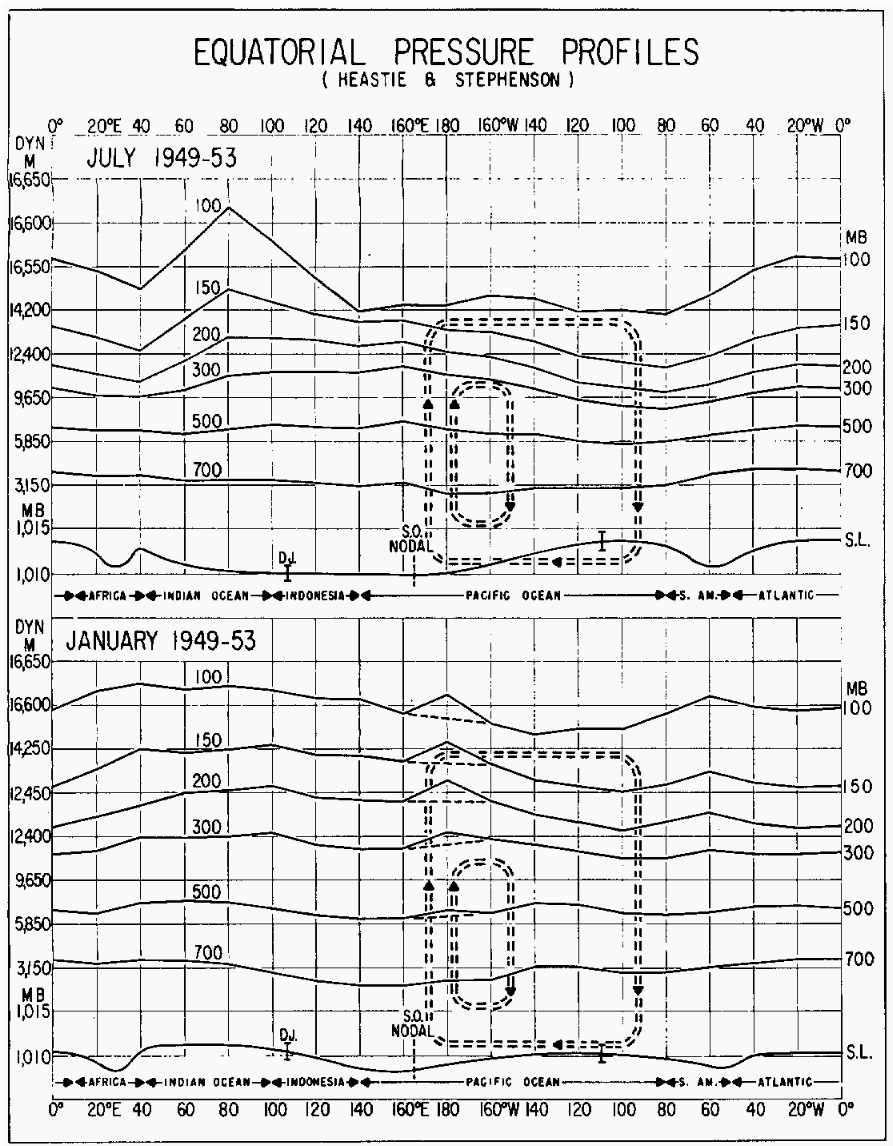
\includegraphics[width=0.9\linewidth]{figures/equatorial-pressure-profiles.png}
  \caption{Height of isobaric streamlines along equator. The \emph{Walker
      circulation} is shown over the Pacific ocean in double-dashed lines, with
    direction indicated by arrows. Source: \citet{bjerknes1969}}
  \label{fig:pressureprofiles}
\end{figure}

Bjerknes states that ``The Walker Circulation ... must be part of the mechanism
of the still larger ``Southern Oscillation'' ...''.

% Diagram here.

%% \cite{bjerknes1969} proposed the currently accepted model for
%% atmospheric circulation driving the SO, calling it the Walker circulation. In
%% this model, dry air sinks over the cool water of the eastern tropical
%% Pacific. After sinking it is transported westward along the equator by the
%% easterly trade winds. As it travels over progressively warmer water the air is
%% warmed and moistened, until it finally reaches the western tropical
%% Pacific. Here the air is now very warm and saturated with water, and it rises in
%% prodigious rain clouds. The circulation is completed with the return flow of air
%% through the upper trophosphere.

%%  % TODO Definitely need some figures here for the Walker circulation.

%% This atmospheric circulation also drives oceanic currents. Water is driven east
%% to west, warming as it goes. This allows for cooler water to rise from the
%% depths along the eastern Pacific, a process called \emph{upwelling}. Combining
%% the oceanic and atmospheric circulations in the Pacific yields a potential
%% explanation for the \elnino\ phenomenon.

\subsection{\elnino-Southern Oscillation}
The Walker circulation requires an east-west tropical Pacific SST gradient for
the transportation of air. An initial positive SST anomaly in the eastern
Pacific ocean would diminish the east-west gradient. A diminished SST gradient
reduces the Walker circulation, in turn weakening the westerly equatorial trade
winds \citep{lindzen1987}. Warm water that was previously being driven westward
by the trade winds can now flow back toward the east, preventing upwelling and
reinforcing the initial SST anomaly. Through positive feedback between the
ocean and the atmosphere, an initial SST anomaly can lead the equatorial Pacific
into a warm state -- \elnino. Since the phenomenon is due to ocean-atmosphere
interaction, the whole system is termed the \elnino-Southern Oscillation
(ENSO). {}\nina\ corresponds to the cold state of ENSO, characterised by
negative SST anomalies and keen trade winds.

%% oscillatory, modes, period

\subsection{Teleconnections}
%take about what drives the teleconnections, i.e. changing circulation
ENSO affects not only the climate of the local Pacific region, but can extend
farther out to influence regions of Africa and Europe \citep{moron1998}. The
magnitude of the influence in these places is of course weaker than locally, but
present nevertheless.

The method by which meteorological influence is communicated between
geographically separated regions is called
\emph{telecommunication}. Telecommunication can proceed via thermal
redistribution between oceans, large-scale transfer of atmospheric energy away
from the equator via the Coriolis force. Bjerknes had described the mechanism by
which anomalous heating of the equatorial Pacific could impart energy into the
Pacific atmosphere and then cause the feedback loop that produces \elnino{}
conditions. The interesting question thereafter is whether ENSO could, by
teleconnection, have effects in remote areas such as Africa and Europe.

Multiple comprehensive studies \citep{ropelewski1987, ropelewski1989,
  nicholson1996} have found that ENSO modulates the rainfall of continental
Africa, although there is some dispute about regional impact
\citep{wolter1989}. Figure \ref{fig:enso_rainfall_anoms} shows the latest
comprehensive study of seasonal rainfall anomalies for ENSO events.

A comprehensive theory of the mechanism of telecommunication has yet to be formed
\citep{philander1990}. One explanation of teleconnection described in
\cite{joly2009} is that anomalous heating of tropical Pacific waters leads to
displacement of the Walker circulation. Recalling that the Walker circulation
has two equatorial areas of action: one of rising moist air in the west, near
South Asia and Australia, and one of descending cool air in the central
Pacific. This circulation is essentially repeated around the equator, with
alternating sites of rising and descending air. When the Walker circulation is
displaced the locations of high precipitation are also shifted. During \elnino{}
the western and eastern Pacific experience less rainfall, with the high
precipitation area moving into the central Pacific. It could then be the case
that the Walker circulation extending over Africa is also shifted -- though less
so -- leading to increased precipitation in some areas, and reduced in others.

\begin{figure*}
  \centering
  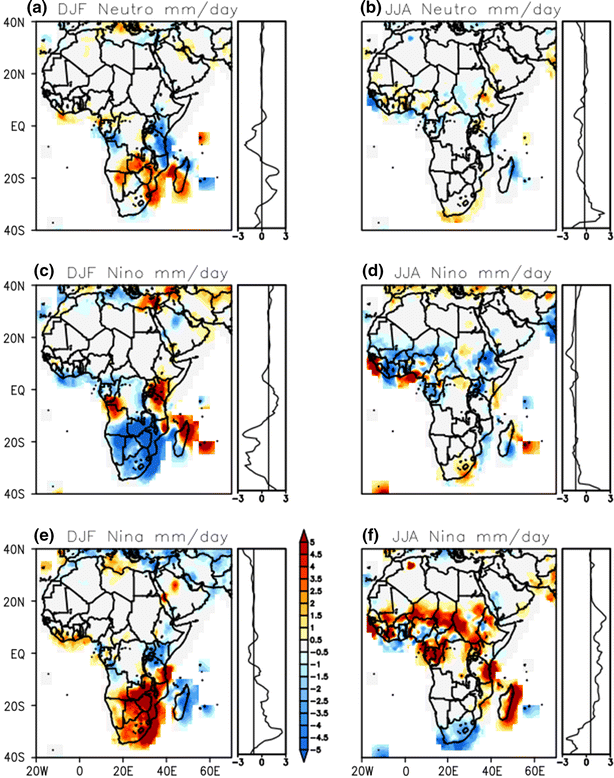
\includegraphics[width=0.7\textwidth]{figures/enso_africa_rainfall_anoms}
  \caption{Distribution of precipitation anomalies and latitudinal averages in
    mm/day, for the DJF and JJA seasons. Panels a) \& b) show neutral years, c)
    \& d) show \elnino\ years and e) \& f) show \nina\ years. The distributions
    show that southern and equatorial Africa exhibit the strongest responses to
    ENSO events, in the DJF and JJA seasons, respectively. DJF corresponds to the
    rainy season and JJA to the dry season for southern Africa and the opposite
    is true for equatorial Africa. Figure taken from \cite{deoliveira2018}.}
  \label{fig:enso_rainfall_anoms}
\end{figure*}

\subsection{Indian Ocean}
On interannual timescales, ENSO is the predominant form of climate variation
\citep{obrien1998}, however it is not the only system that can affect weather on
the African continent. An ocean-atmosphere mode in the Indian Ocean, caused by
anomalously high (low) sea surface temperatures in the western (eastern) regions
of the ocean, was identified by \cite{saji1999} and is starting to be considered
as an influential player in climate dynamics. \cite{anyamba2002} suggest that
the observed vegetation response in regions of Africa between $1997-2000$ was
more significantly driven by these western Indian Ocean SST anomalies, than
anomalies in the Pacific. This mode, called the Indian Ocean Dipole (IOD) has
also been linked to the `Big Dry' -- the severe drought that has been ongoing in
southern Australia since 1995 \citep{karumuri2003, ummenhofer2009}.

Furthermore, the effects of the IOD are not solely continental -- there is
evidence to suggest that the IOD can be involved with the ENSO itself. There
have been multiple studies into its role as a contributor to both the growth
\citep{annamalai2005, hackert2017} and demise \citep{okumura2010, kug2006,
  xie2009, dayan2015} of \elnino{} events. \cite{dong2018} propose that not only
can the IOD influence an established \elnino{} event, but that it may in fact be
able to stop an \elnino{} event developing at all. It follows, then, that in
order to better predict \elnino{} events we must take the Indian Ocean into
account \citep{hackert2017}.

\subsection{Cloud Coverage}
\label{sec:intro:cc}
Cloud coverage calculations are an important part of climate science owing in no
small part to their effects on human life. Clouds bring precipitation and
precipitation brings flourishing vegetation. Prolonged periods of rainfall can,
however, cause perilous floods which can ruin infrastructure and produce,
endangering lives. Conversely, periods with little rainfall can cause
catastrophic drought, such as that currently seen in Cape Town, South Africa,
where useful water is soon expected to be completely depleted. Either way, cloud
coverage has a major impact on human life and is deserving of careful
observation and examination.

Cloud coverage analyses have historically been based upon land-based
observations. New analysis methods were developed with the advent of remote
sensing data, the most common of which is based on thresholding. For example,
\cite{derrien1993} employ thresholds determined from monthly SST measurements
where the thresholds themselves are temperatures, as opposed to pixel values. In
our analysis, we have hypothesised using the bimodality of the distribution of pixel
values to facilitate our thresholding, the validity of which is discussed in
Section \ref{sec:disc:thresh}.

\cite{warren2007} looked at cloud cover and cloud type variation in the period
1971--1976. A large interannual change was found for Australia, with a small but
statistically significant change found for Africa. This result suggests
motivation for our work focusing on the effect of ENSO (which is known to affect
Australia) upon Africa. Monthly and yearly averages were taken in order to
diminish small-scale variation.

\subsection{Normalised Difference Vegetation Index}
\label{sec:intro:ndvi}
%% Use \cite{yengoh2014}, \cite{bannari1995}, and lit reviews.
Green vegetation has a distinctive spectral response to electromagnetic
radiation. Near infra-red radiation is strongly reflected by green leaf
surfaces, while the chlorophyll within the leaves absorbs strongly in the
red. Figure \ref{fig:leaf_spec} shows the spectral reflectance for green
vegetation, dry soil and wet soil, where the reflectance in the near infrared
and absorption in the read are clearly visible.
\begin{figure}
  \centering
  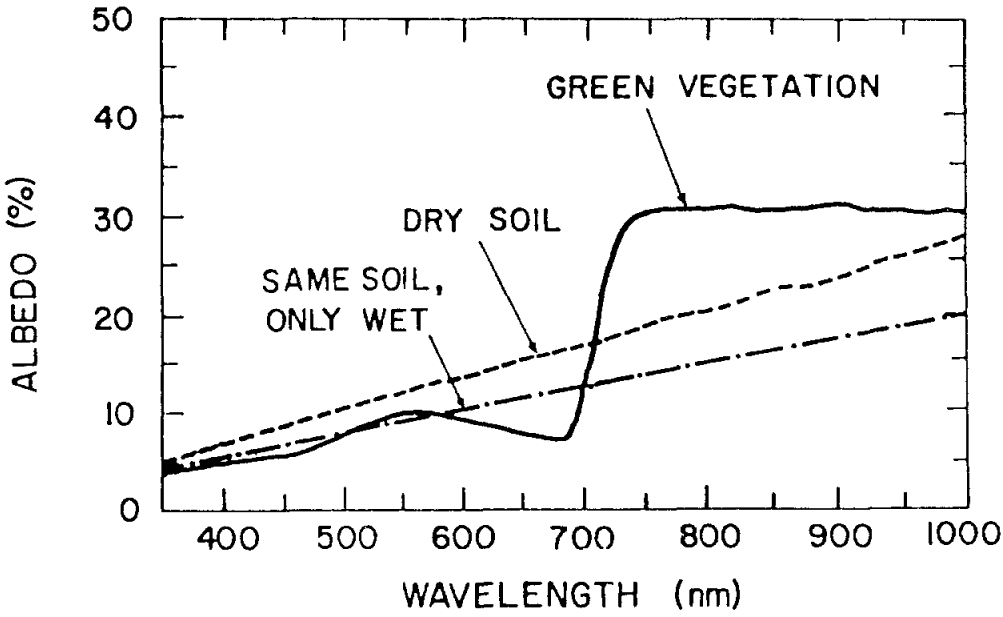
\includegraphics[width=0.9\linewidth]{figures/leaf_spec}
  \caption{Spectral response of green vegetation, dry soil and wet soil. Note how green vegetation is highly absorbing in the red and highly reflecting in the infra-red. Figure taken from \cite{tucker1977}.}
  \label{fig:leaf_spec}
\end{figure}
Hence we determine vegetation coverage using the normalised difference
vegetation index (NDVI) defined as
\begin{equation}
  \mathrm{NDVI} = \frac{\rho_{\mathrm{NIR}}-\rho_{\mathrm{R}}}{\rho_{\mathrm{NIR}}+\rho_{\mathrm{R}}}
  \label{eq:ndvi}
\end{equation}
where $\rho_{\mathrm{NIR}}$ and $\rho_{\mathrm{R}}$ are the reflectances in the
near-infrared and red bands respectively \citep{tucker1979}.

\cite{nicholson1990} found that there is a strong spatial correlation between
NDVI values integrated over a year and average annual rainfall. The same study
also found that, on interannual and seasonal timescales, variability in rainfall
is mirrored in NDVI. Figure \ref{fig:ndvi_rain} shows the spatial correlation of
rainfall and NDVI, displaying the spatial correlations described in
\cite{nicholson1990}.
\begin{figure}
  \centering
  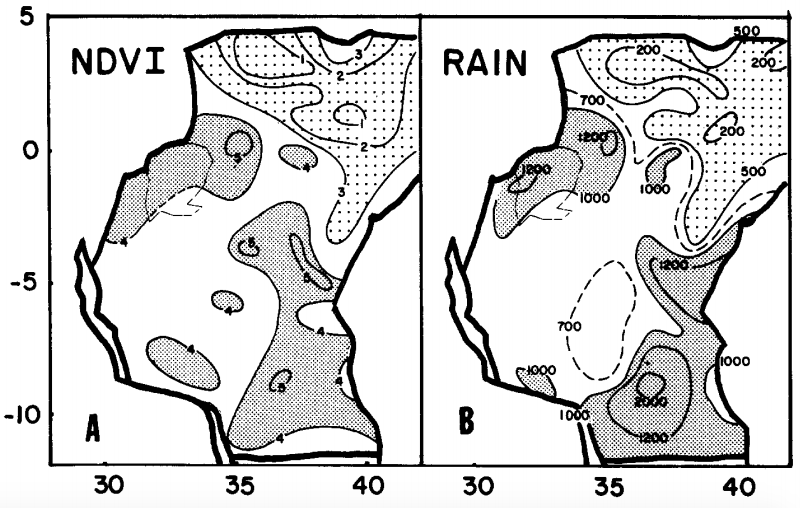
\includegraphics[width=0.9\linewidth]{figures/ndvi_rain}
  \caption{Left: annual integrated NDVI for East Africa averaged over 1982--1985,
    shading indicates NDVI ${>}4$ and dotting indicates NDVI ${<}3$. Right: mean
    annual rainfall in mm over the period 1982--1985, shading indicates rainfall
    ${>}1000$ mm/year and dotting indicates rainfall ${<}500$ mm/year. Figure
    taken from \cite{nicholson1990}.}
  \label{fig:ndvi_rain}
\end{figure}
%% Local Variables:
%% fill-column: 80
%% TeX-master: "report"
%% End:
